\section{Functies en afgeleiden}



\subsection{Functies}

Eén van de centrale concepten binnen de wiskunde, en zeker zeker ook binnen de \textit{machine learning} is de \textit{functie}. Formeel beschrijft een functie een relatie tussen twee verzamelingen $X$ en $Y$, waarbij een element uit $X$ gekoppeld wordt aan precies één element uit de verzameling $Y$. Eenvoudiger gezegd is een functie een verhouding tussen twee getallen, waarbij het ene getal (de zogenaamde \textit{afhankelijke variabele}) wordt uitgedrukt in termen van het andere getal (de \textit{onafhankelijke variabele}). Je kunt een functie opvatten als een machine die een geschikte invoer (geschikte getallen) omzet in een bepaalde uitvoer.

Een functie in de wiskunde doet op deze manier denken aan een functie (of \textit{methode}) zoals we die kennen uit onze programmeerervaring. Zo wordt door de Java-methode \texttt{subString} een string omgezet in een betreffende substring, maar alleen als je deze aanroept met twee parameters van het type \texttt{int}. In methoden of functies waarin geen waarde wordt geretourneerd, is het return statement impliciet (elke methode of functie retourneert dus uiteindelijk een waarde).

In de regel wordt de ongebonden variabele aangegeven met $x$ en de gebonden variabele met $y$. Om aan te geven dat $y$ van $x$ afhankelijk is, schrijf je de \textit{vergelijkingsvorm} $y=formule$, bijvoorbeeld $y=2x+3$. Een andere notatievorm is de \textit{haakjesvorm}: $f(x) = 2x+3$ – de functiewaarde van $y$ is gelijk aan $2x+3$. Behalve het geven van een formule kun je een functie natuurlijk ook in een assenstelsel tekenen. Hierbij zetten we de $x$ op de horizontale lijn en de $y$ op de verticale lijn. Elk punt in onze formule geven we dan weer als het \textit{tupel} $(x,y)$. Door al deze punten met elkaar te verbinden, verkrijgen we de grafiek van onze functie:

\begin{figure}[h]
    \centering
    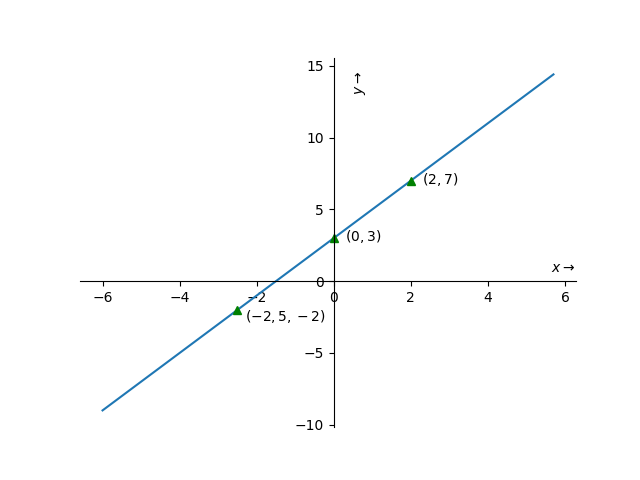
\includegraphics[width=.75\textwidth]{functie}
    \caption{Voorbeeld van een grafiek van een functie.\label{img:functie}}
\end{figure}

De verzameling van alle mogelijke waarden van de ongebonden variabele (de \textit{input}) is het \textit{domein} van de functie, dat we aangeven met $D$; de verzameling van de mogelijke waarden van de gebonden variabele (de \textit{output}) is het \textit{bereik} van die functie, wat wordt weergegeven met $B$. Gegeven een functie $f(x)=\sqrt{x-1}$, dan is het \textit{domein} van die functie de verzameling van alle getallen groter dan of gelijk aan 1, terwijl het \textit{bereik} van die functie gelijk is aan alle getallen groter dan of gelijk aan 0. Een dergelijke verzameling van getallen kun je omschrijven als een \textit{interval}: als $a < b$ dan vormen alle getallen tussen $a$ en $b$ het \textit{open interval} $\left<a,b\right>$. Als de getallen $a$ en $b$ ook bij het interval horen, dan spreek je van een \textit{gesloten interval}, wat je schrijft als $\left[a,b\right]$.

Een functie kan op een bepaald interval \textit{stijgen}, \textit{dalen}, of \textit{gelijk blijven}. Een stijging of daling kan constant zijn, toenemen of afnemen. Het punt waarop een functie van een stijging overgaat naar een daling heet een \textit{maximum}; het punt waar een functie overgaat van een daling naar een stijging heel een \textit{minimum}. Zo heeft de functie in Figuur \ref{img:min_max} een maximum in punt $(A, f(A))$ en een minumum in punt $(B, f(B))$. De functie vertoont een \textit{afnemende stijging} tussen $\left[-\infty, A \right>$ en een \textit{toenemende stijging} tussen $\left< B, \infty \right]$; hij \textit{daalt} tussen $\left[A,B\right]$. Verder is zowel het \textit{domein} als het \textit{bereik} van deze functie $\left[-\infty, \infty\right]$.

\begin{figure}[h]
\centering
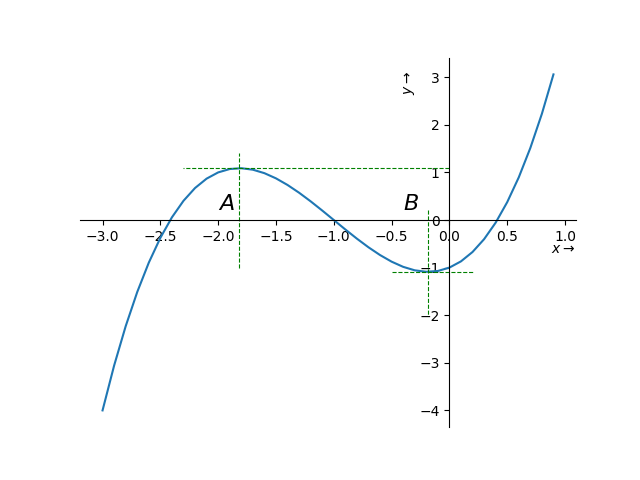
\includegraphics[width=.75\textwidth]{min_max}
\caption{Een functie met een minumum en een maximum.\label{img:min_max}}
\end{figure}

\subsection{Machtfuncties en polynomen}

Een \textit{machtsfunctie} is een functie waarvan de algemene vorm $f(x)= a \cdot x^n$ is, waarbij $a$ (de \textit{vermenigvuldigingsfactor} en $n$ (de \textit{exponent}) willekeurige positieve of negatieve getallen kunnen zijn. Wanneer de exponent geen geheel getal is, mag $x$ niet negatief zijn. Wanneer de exponent een negatief getal is, mag $x$ niet 0 zijn. 

In Figuur \ref{img:machtsfuncties} zijn de grafieken van $x^2$ (blauwe lijn), $x^3$ (groene stippellijn), $x^4$ (rode lijn) en $x^5$ (magenta stippellijn) getekend. Als je goed naar deze grafieken kijkt, valt een aantal zaken op. Alle vier de functies gaan door de punten $(0,0)$ en door $(1,1)$. Het bereik van de functies waarvan de exponent een \textit{even getal} is, ligt boven de y-as ($f(x) \geq 0$ voor alle $x \in D$) en deze functies zijn \textit{lijnsymmetrisch} in de y-as (dus $f(-x) = f(x)$ voor alle $x \in D$). Verder gaan deze functies allemaal door het punt $(-1, -1)$. De functies waarvan de exponent een \textit{oneven getal} is, gaan allemaal door punt $(-1,-1)$ en zijn \textit{puntsymmetrisch} in punt $(0,0)$ (dus $f(-x)=-f(x)$ voor alle $x \in D$).

\begin{figure}[h]
    \centering
    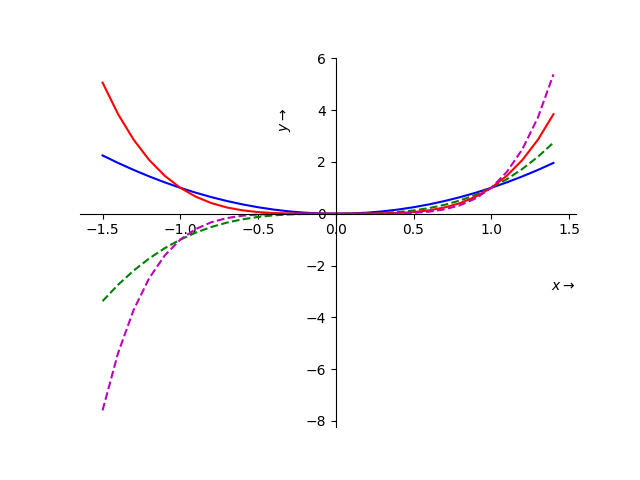
\includegraphics[width=.75\textwidth]{machtsfuncties}
    \caption{Diverse machtsfuncties bij elkaar getekend.\label{img:machtsfuncties}}
\end{figure}

Vaak zie je, zeker in het geval van machine learning, dat een functie bestaat uit een aantal termen met verschillende machten, zoals bijvoorbeeld de functie $f(x) = x^3+3x^2+2x$, die is weergegeven in Figuur \ref{img:polynoom}. Zo'n soort functie noemen we een \textit{polynoom} (van het Griekse polús (veel) en nomós (deel): een functie die uit veel delen bestaat). Je ziet hier dat $f(x)=0$ voor $x=-2$, $x=-1$ en $x=0$ (de \textit{nulpunten}). Verder zitten er  tussen de nulpunten een minimum en een maximum (hoewel die niet exact midden tussen de nulpunten in liggen). Wanneer we waarden van $x$ nemen die heel groot of heel klein zijn, heeft de hoogste term in de functie-definitie de sterkste invloed op de waarden van $f(x)$ – de functie gaat nagenoeg gelijk lopen met de functie $g(x)=x^3$. Alleen dicht bij de 0 zijn er wat verschillen waar te nemen. Deze functie wordt een om die reden een polynoom van de \textit{derde graad} genoemd: de hoogste exponent van de functie-definitie bepaalt de \textit{graad} van de functie. 


\begin{figure}[h]
    \centering
    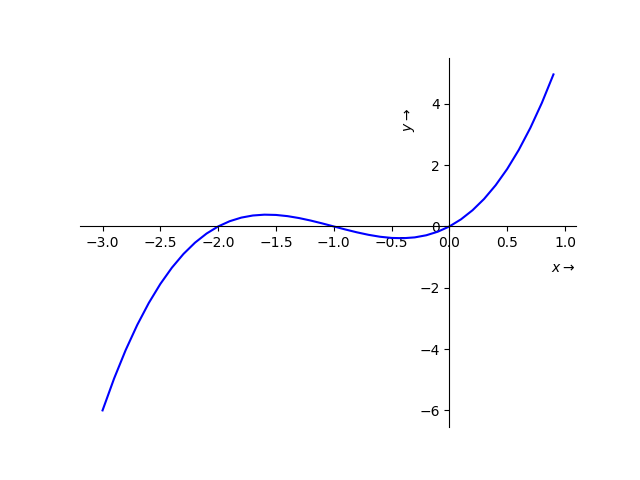
\includegraphics[width=.75\textwidth]{polynoom}
    \caption{Een polynoom van de derde graad.\label{img:polynoom}}
\end{figure}

Net als bij enkelvoudige functies kunnen de termen in een polynoom voorzien worden van een vermenigvuldigingsfactor. Zo heeft de term $x^2$ in de polynoom in Figuur \ref{img:polynoom} een vermenigvuldigingsfactor van 3 en de term $x$ een vermenigvuldigingsfactor van 2 (feitelijk is de vermenigvuldigingsfactor van de term $x^3$ gelijk aan 1, dus dat laten we weg). Het is gebruikelijk om voor het beschrijven van deze factoren dezelfde letter te gebruiken, en die te voorzien van de term waar deze bij hoort als subscript. Zo wordt de algemene beschrijving van een polynoom gegeven door $f(x) = a_nx^n + a_{n-1}x^{n-1} + a_{n-2}x^{n-2}+ \dots + a_1x^1+a_0$: dit is dan een polynoom van de n-de graad.


\subsection{Afgeleide functies}

Vaak is het van belang om te weten of een functie op een interval $\left[a,b\right]$ stijgt of daalt – de zogenaamde \textit{differentie}. Om dit te bepalen, kunnen we de waarde van $f(x)$ (of $y$) voor zowel $a$ als $b$ uitrekenen en van elkaar aftrekken. Als $f(a) < f(b)$, dan is de differentie van $f(x)$ op $\left[a,b\right]$ \textit{negatief}: de functie vertoont een daling op het interval. Omgekeerd, als $f(a) > f(b)$, dan is de differentie van $f(x)$ op $\left[a,b\right]$ \textit{positief}: de functie vertoont een stijging. De totale differentie geven we aan met de griekse hoofdletter delta: \Delta.

In Figuur \ref{img:hyperbool} is de functie $f(x) = \frac{1}{4x}$ op het interval $\left<0,2\right]$ weergegeven. Stel dat we de daling van deze functie op het interval $\left[\frac{1}{8}, \frac{1}{4}\right]$ willen weten, zoals aangegeven door de linker groene stippellijn. Om dit te bepalen, berekenen we eerst $f(x)$ voor het rechter extreem van het interval, en trekken daar $f(x)$ voor het linker extreem vanaf. De totale daling $\Delta$ wordt dan $f(\frac{1}{4}) - f(\frac{1}{8}) = \frac{1}{1} - \frac{1}{0.5} = 1 - 2 = -1$. Op eenzelfde manier kunnen we de totale differentie op het interval $\left[\frac{1}{4},1\right]$ bepalen: $\Delta = f(1) - f(\frac{1}{4})  = \frac{1}{4} - \frac{1}{1} = 0.25 - 1 = -0.75$.

\begin{figure}[h]
    \centering
    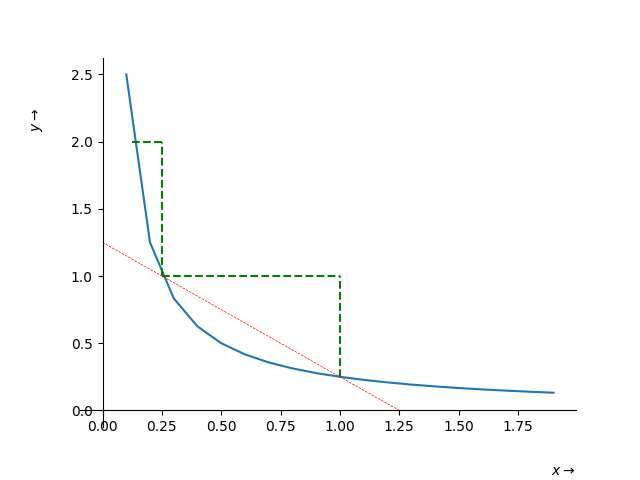
\includegraphics[width=.75\textwidth]{hyperbool}
    \caption{De functie $f(x) = 1/4x$\label{img:hyperbool}}
\end{figure}
    
Behalve het totaal is ook de \textit{gemiddelde} stijging of daling van belang – het zogenaamde \textit{differentiequotiënt}. Dit berekenen we door de totale stijging of daling op een interval te delen door de lengte van het interval. Het differentiequotiënt van $f(x)$ uit Figuur \ref{img:hyperbool} op het interval $\left[\frac{1}{4},1\right]$ is dus $\frac{-0.75}{1-\frac{1}{4}} = -1$. Dit cijfer correspondeert met de \textit{richtingscoëfficiënt} van de lijn die de beide extremen van het gegeven interval met elkaar verbindt – de rode stippellijn in Figuur \ref{img:hyperbool}. Algemeen geldt dat als $a<b$, het differentiequotiënt gelijk is aan

\[
    \frac{f(b)-f(a)}{b-a}.
\]


Om de differentie van een functie op een specifiek punt $f(a)$ te bepalen, berekenen we de gemiddelde differentie van de functie op het interval $\left[a,a+h\right]$, waarbij we $h$ steeds kleiner maken. Stel nu dat $f(x)=x^2$, dan kunnen we differentie op punt $x$ als volgt bepalen:
\[
\begin{aligned}
    \Delta &= \frac{f(x+h)-f(x)}{(x+h) - x} & \text{waarden voor } x \text{ en } h \text{ invullen:}\\
    &= \frac{(x+h)^2 - x^2}{(x+h)-x} & \text{kwadraten uitwerken en noemer versimpelen:} \\
    &= \frac{(x^2 + 2xh + h^2)-x^2}{h} & \text {teller vereenvoudigen:} \\
    &= \frac{2xh + h^2}{h} & \text{alles delen door h:} \\
    &= 2x + h & \text{h nadert tot nul:} \\
    &= 2x
\end{aligned}
\]            

We zien dus dat de differentie van elk punt $x$ op de functie $f(x) = x^2$ zelf ook weer een functie van $x$ is, namelijk $2x$. 
Deze tweede functie heet de \textit{afgeleide functie} van $f(x)$ en wordt genoteerd als $f'(x)$, of als een zogenaam \textit{differentiequotiënt}:

\[
    f'(x) = \frac{df}{dx}
\]

Het bepalen van een afgeleide functie wordt \textit{differentiëren} genoemd; de grafiek van $f'(x)$ heet de \textit{hellingsgrafiek} van $f(x)$. Differentiëren is een tak van de wiskunde die behoorlijk complex kan worden, maar voor nu volstaan de volgende algemene regels:

\begin{itemize}
    \item De hellingsgrafiek van de functie $f(x)=0$ is de lijn $f'(x)=0$: de verandering is overal 0.
    \item De hellingsgrafiek van een constante functie $f(x)=x$ is de lijn $f'(x)=1$: de verandering blijft overal hetzelfde.
    \item De hellingsgrafiek van een niet-horizontale lijn $f(x) = ax + b$ is de constante functie $f'(x)=a$: het lokale verandering van functiewaarden is overal hetzelfde. 
    \item In het algemeen geldt dat als $f(x) = x^n$, dan is $f'(x) = nx^{n-1}$. 
\end{itemize}

Wanneer we een functie $f(x)$ met domein $D$ hebben, noemen we deze functie \textit{differentieerbaar} wanneer we voor elke $x \in D$ een afgeleide waarde kunnen bepalen. Zo is de functie $f(x) = x^2$ differentieerbaar, want over het hele domein ($D = \left[-\infty, \infty\right]$) kunnen we een afgeleide waarde bepalen, namelijk $f'(x)=2x$. De functie $f(x)=|x|$ (zie Figuur \ref{img:abs}) is daarentegen niet differentieerbaar: de afgeleide functie hiervan is $f'(x)=-1 (x<0)$ en $f'(x)=1 (x>0)$, maar voor $x=0$ is de afgeleide waarde ongedefinieerd: je kunt immers oneindig veel lijnen trekken die allemaal het punt $(0,0)$ raken (in de figuur zijn twee voorbeelden getekend – de groene stippellijnen).

\begin{figure}[h]
    \centering
    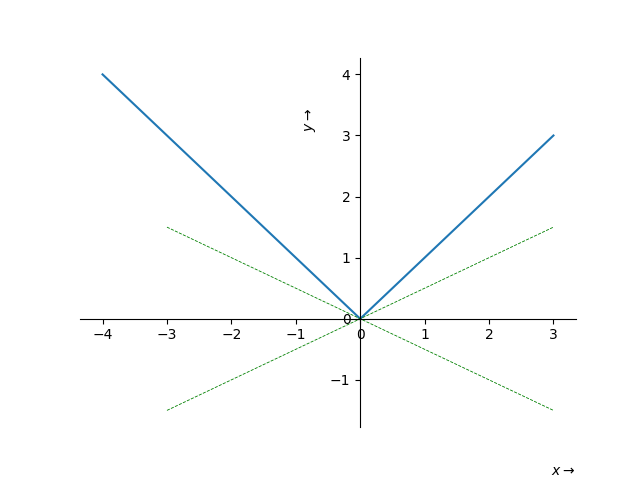
\includegraphics[width=.75\textwidth]{absoluut}
    \caption{De functie $f(x) = |x|$\label{img:abs}}
\end{figure}
